\documentclass{article}
\newcommand\tab[1][1cm]{\hspace*{#1}}

\usepackage{hyperref}
\usepackage{graphicx}
\usepackage{caption}

\hypersetup{colorlinks=false,
	allbordercolors={0 0 0},
	pdfborderstyle={/S/U/W 1}
}

\title{COMP SCI 5401 FS2016 Assignment 2c}
\author{Robert Jones \\ \href{mailto:rbj2q2@mst.edu}{rbj2q2@mst.edu} }
\date{\today}


\begin{document}

\maketitle

\tableofcontents

\clearpage
\section{Experiment Comparisons}
\subsection{Methodology}
\begin{flushleft}
For this experiment, both pac controllers and ghost controllers are evolved in
 competitive co-evolution. All parameters for evolution of both populations are
 independent and the fitnesses of pac and ghosts are related to the scores in
 mutual games the pacs get; Where pac score positively affects pac fitness,
 it negatively affects ghost fitness. Additionally, pac and ghosts are evaluated
 in a shared game instance. All population members have to be re-evaluated each
 generation.

 \tab
For this group of experiments, the mutation rate was experimented on to find
 the optimal rate. The tested rate are 10%, 50% and 90%. 50% is designated as
 the base for all other experiments. It is expected that 50% will at least be
 decent, where the other two are potentially destructive.
\end{flushleft}
\subsection{Experimental Setup}
\begin{flushleft}
EA parameters were chosen to be as close as possible to the default
 configuration to minimize changes caused by other forces. In other words, the
 only variable desired was the variable being tested. The variable parameter was
 chosen as such to match expectations for the assigned bonus. The random number
 value was seeded randomly.

\tab
In terms of algorithms, this experimentconsisted of vectors of each population
 that are tested concurrently. Trees are nearly identical in terms of sensors,
 except that the ghost controllers do not have wall, pill or fruit sensors.
 Scores for pac controllers scale positively with game score, while ghost
 controllers scale negatively with pac scores. Ramped Half-and-Half
 initialization is used. Over-Selection is used for parent selection, sub-tree
 crossover is used for recombination, and sub-tree mutation is used for
 mutation. Truncation is used for survival selection and parsimony pressure is
 used for bloat control. The only termination condition is number of
 evaluations, which is 2000 per run with 30 runs per experiment.
\end{flushleft}

\clearpage
\subsection{Results}
\begin{flushleft}
\begin{figure}[h]
	\centering
	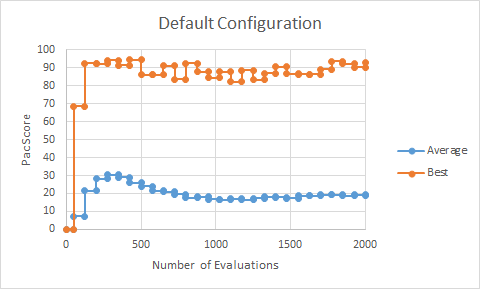
\includegraphics[width=0.8\textwidth]{default}
	\caption{Results of Default Configuration}
\end{figure}

\begin{figure}[h]
	\centering
	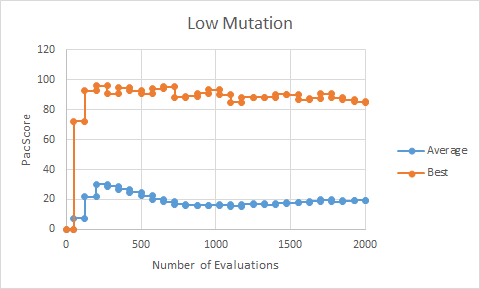
\includegraphics[width=0.8\textwidth]{lowMut}
	\caption{Results of Low Mutation Configuration}
\end{figure}
\end{flushleft}

\clearpage

\begin{flushleft}
\begin{figure}[h]
	\centering
	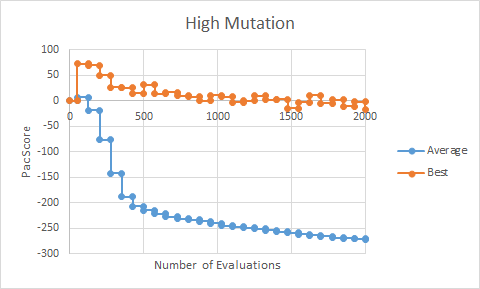
\includegraphics[width=0.8\textwidth]{highMut}
	\caption{Results of High Mutation Configuration}
\end{figure}

\vspace{15mm}

\begin{figure}[h]
	\centering
	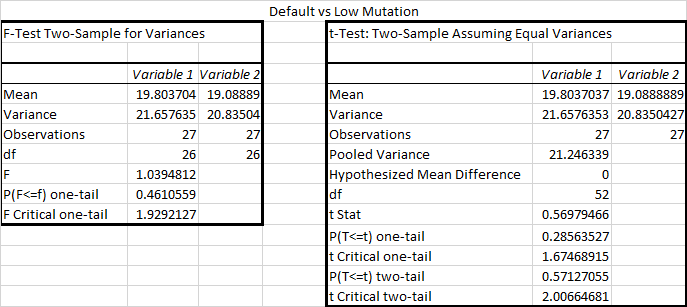
\includegraphics[width=0.8\textwidth]{statDefaultVsLowMut}
	\caption{Statistical Analysis of Default Configuratin vs Low Mutation}
\end{figure}
\end{flushleft}

\clearpage

\begin{flushleft}
\begin{figure}[h]
	\centering
	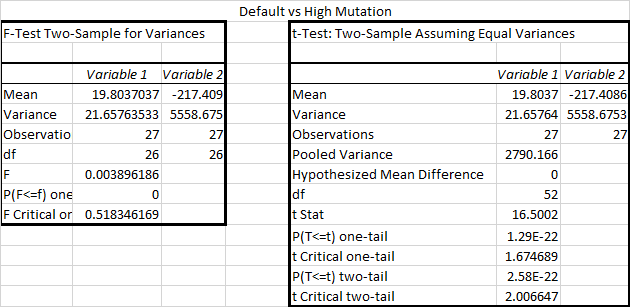
\includegraphics[width=0.8\textwidth]{statDefaultVsHighMut}
	\caption{Statistical Analysis of Default Configuratin vs High Mutation}
\end{figure}

\vspace{15mm}

\begin{figure}[h]
	\centering
	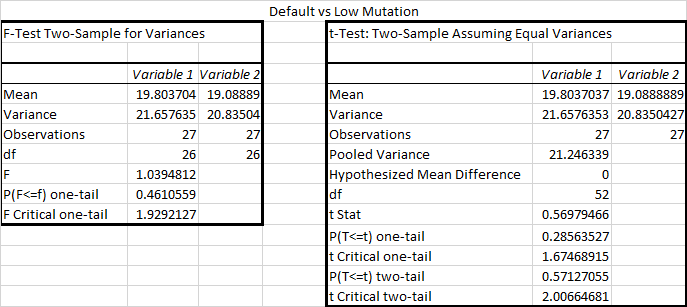
\includegraphics[width=0.8\textwidth]{statDefaultVsLowMut}
	\caption{Statistical Analysis of Low Mutation vs High Mutation}
\end{figure}
\end{flushleft}

\clearpage
\subsection{Discussion}
\begin{flushleft}
\tab
The mean of the basic configuration is greater than the mean of the low mutation
 configuration, and F is less than F Critical,
 so equal variances can be assumed. The absolute value of T stat is less than the
 absolute value of t critical two-tail, so it can not be determined with 95%
 confidence whether either configuration is better.

\tab
The mean of the basic configuration is greater than the mean of the high
 mutation configuration, and F is less than F Critical,
 so equal variances can be assumed. The absolute value of T stat is greater
 than the absolute value of t critical two-tail, so it can be stated with 95%
 confidence that using the high mutation configuration is less evolutionarily
 advantageous for pac controllers than the basic configuration.

\tab
The mean of the low mutation configuration is greater than the mean of the high
 mutation configuration , and F is less than F Critical,
 so equal variances can be assumed. The absolute value of T stat is greater
 than the absolute value of t critical two-tail, so it can be stated with 95%
 confidence that using the high mutation configuration is less evolutionarily
 advantageous for pac controllers than the low mutation configuration.
\end{flushleft}


\subsection{Conclusion}
\begin{flushleft}
The high mutation configuration is markedly worse than the base configuration
 and the low mutation configuration. It is possible that the high mutation rate
 is more beneficial for a smaller number of terminal options. In this case, the
 ghost controller would have an advantage, which would explain the behavior of
 the high mutation graph, where ghost controllers quickly dominate the pac
 controllers. As such, increasing the mutation rate can be an extremely useful
 tool when a population with small trees needs to be pushed towards equilibrium
 with a population with larger trees that are dominant.
\end{flushleft}

\clearpage
\section{Bonus 1}
\subsection{Methodology}
\begin{flushleft}
For this experiment, a unique ghost controller was used for each ghost. To do
this, a vector of different ghosts is used and passed in until the limit of
ghosts is reached. The results are then recorded and compared against a
configuration file with the same parameters except it doesn't have unique ghost
controllers.
\end{flushleft}

\subsection{Experimental Setup}
\begin{flushleft}
EA parameters were chosen to be as close as possible to the default
configuration to minimize changes caused by other forces. In other words, the
only variable desired was the variable being tested. The variable parameter was
chosen as such to match expectations for the assigned bonus. The random number
value was seeded randomly.
\end{flushleft}

\clearpage
\subsection{Results}
\begin{flushleft}
\begin{figure}[h]
	\centering
	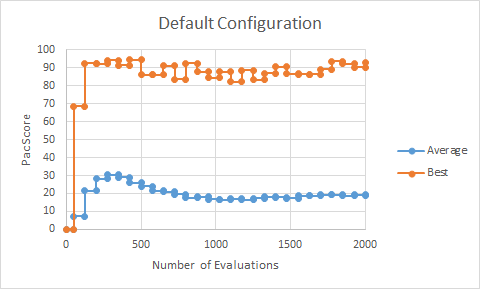
\includegraphics[width=0.8\textwidth]{default}
	\caption{Results of Default Configuration}
\end{figure}

\begin{figure}[h]
	\centering
	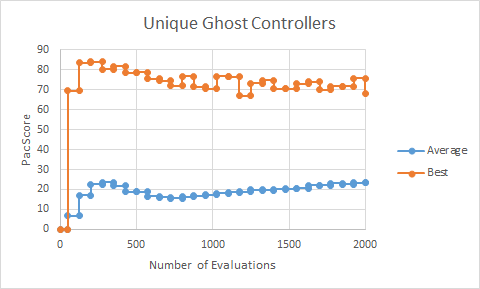
\includegraphics[width=0.8\textwidth]{uniqueGhost}
	\caption{Results of Configuration with Unique Ghost Controller}
\end{figure}
\end{flushleft}

\clearpage

\begin{flushleft}
\begin{figure}[h]
	\centering
	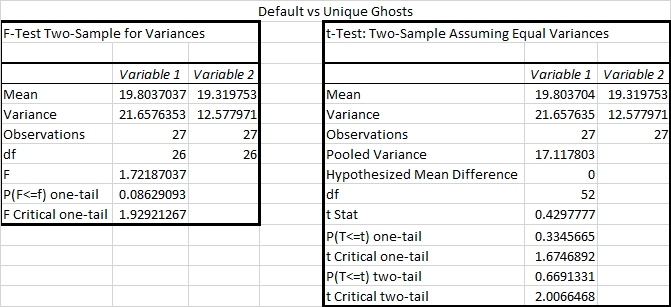
\includegraphics[width=0.8\textwidth]{statDefaultVsUniqueGhost}
	\caption{Statistical Analysis of Default Configuration vs Configuration with Unique Ghost Controllers}
\end{figure}
\end{flushleft}

\subsection{Discussion}
\begin{flushleft}
The mean of the default configuration is less than the mean of the configuration
 with ghost controllers, and F is less than F Critical, so equal variances can
be assumed. The absolute value of T stat is less than the absolute value of t
critical two-tail, so it can not be determined with 95% confidence whether
either configuration is better.

\tab
However, the curve of the unique ghost controller shows a gradual lowering of
the best pac controller. However, the average of pac controllers continued to
increase for average pac controller fitness. This combination of weakening the
most fit individual but allowing an increase in the average could show
more successful co-evolution.
\end{flushleft}

\subsection{Conclusion}
\begin{flushleft}
In conclusion, both same and unique ghost controllers have strengths and
weaknesses that appear to balance each other out. It may be beneficial to use
both forms of controller usage. This should be investigated for meta-EAs.
\end{flushleft}

\clearpage
\section{Bonus 2}
\subsection{Methodology}
\begin{flushleft}
For this experiment, two pac men were used in conjunction with three ghosts per
 game. Each game will only end when both pac are killed by a ghost. To improve
 pac ability to coordinate, a sensor was added in pac controllers that detects
 the distance to another pac. Experiments without unique controllers, with only
 unique pac controllers, with only unique ghost controllers, and with both both
 populations having unique controllers.
\end{flushleft}
\subsection{Experimental Setup}
\begin{flushleft}
EA parameters were chosen to be as close as possible to the default
 configuration to minimize changes caused by other forces in the event that
 comparison to the default was desired. In other words, the only variables
 desired were the variables being tested. The variable parameter was chosen as
 such to match expectations for the assigned bonus. The random number value was
 seeded randomly.
\end{flushleft}

\clearpage
\subsection{Results}
\begin{flushleft}
\begin{figure}[h]
	\centering
	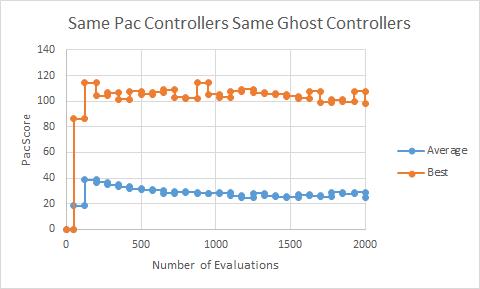
\includegraphics[width=0.8\textwidth]{samePacSameGhost}
	\caption{Results of Default Configuration with 2 Pac}
\end{figure}

\begin{figure}[h]
	\centering
	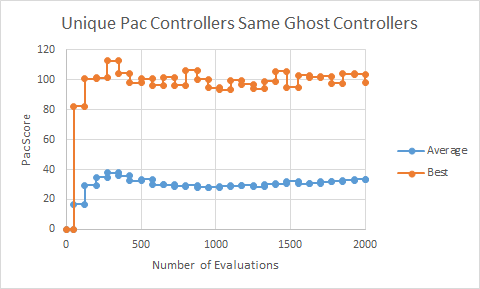
\includegraphics[width=0.8\textwidth]{diffPacSameGhost}
	\caption{Results of Configuration with 2 Unique Pac Controllers}
\end{figure}
\end{flushleft}

\clearpage

\subsection{Results}
\begin{flushleft}
\begin{figure}[h]
	\centering
	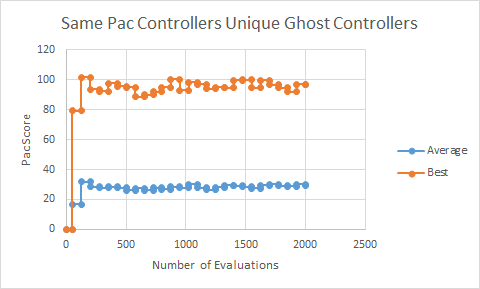
\includegraphics[width=0.8\textwidth]{samePacDiffGhost}
	\caption{Results of Default Configuration with 2 Pac and Unique Ghost Controllers}
\end{figure}

\begin{figure}[h]
	\centering
	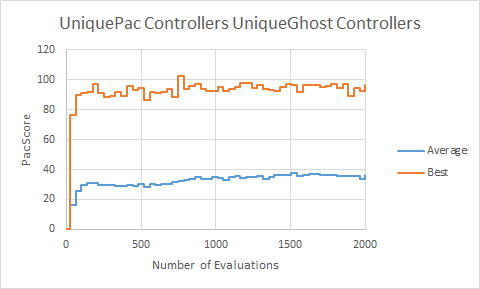
\includegraphics[width=0.8\textwidth]{diffPacDiffGhost}
	\caption{Results of Configuration with 2 Unique Pac Controllers and Unique Ghost Controllers}
\end{figure}
\end{flushleft}

\clearpage

\begin{flushleft}
\begin{figure}[h]
	\centering
	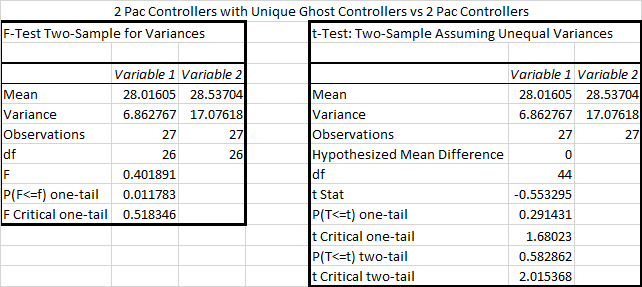
\includegraphics[width=0.8\textwidth]{stats2UniqueGhostVsDefault}
	\caption{Statistical Analysis of Unique Ghost Controllers vs Basic}
\end{figure}

\vspace{15mm}

\begin{figure}[h]
	\centering
	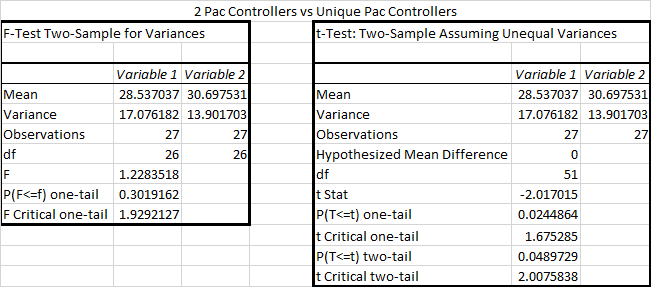
\includegraphics[width=0.8\textwidth]{stats2VsUniquePac}
	\caption{Statistical Analysis of Basic vs Unique Pac Controllers}
\end{figure}
\end{flushleft}

\clearpage

\begin{flushleft}
\begin{figure}[h]
	\centering
	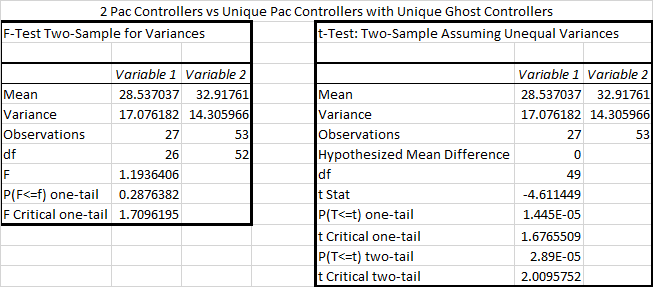
\includegraphics[width=0.8\textwidth]{stats2VsUniquePacAndUniqueGhost}
	\caption{Statistical Analysis of Basic vs Unique Ghost and Pac Controllers}
\end{figure}

\vspace{15mm}

\begin{figure}[h]
	\centering
	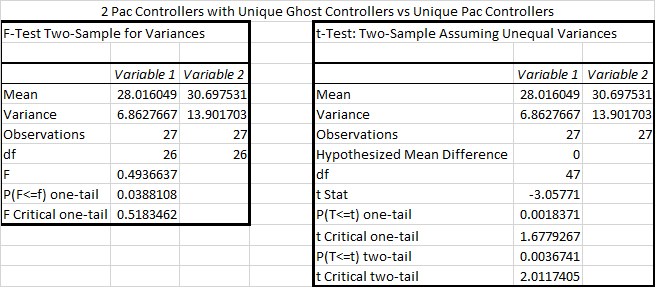
\includegraphics[width=0.8\textwidth]{stats2UniqueGhostVsUniquePac}
	\caption{Statistical Analysis of Unique Ghost Controllers vs Unique Pac Controllers}
\end{figure}
\end{flushleft}

\clearpage

\begin{flushleft}
\begin{figure}[h]
	\centering
	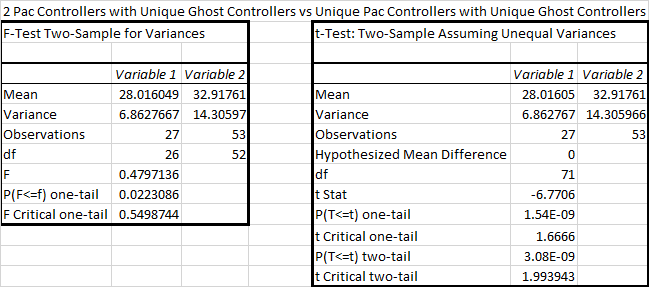
\includegraphics[width=0.8\textwidth]{stats2UniqueGhostVsUniquePacAndGhost}
	\caption{Statistical Analysis of Unique Ghost Controllers vs Unique Ghost and Pac Controllers}
\end{figure}

\vspace{15mm}

\begin{figure}[h]
	\centering
	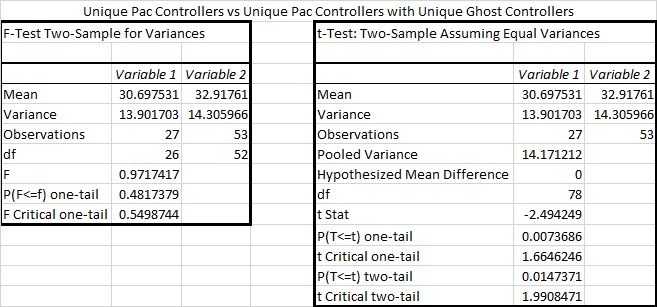
\includegraphics[width=0.8\textwidth]{stats2UniquePacVsUniquePacAndUniqueGhost}
	\caption{Statistical Analysis of Unique Pac Controllers vs Unique Ghost and Pac Controllers}
\end{figure}
\end{flushleft}

\clearpage
\subsection{Discussion}
\begin{flushleft}
\tab
The mean of the basic configuration is greater than the mean of the
configuration with unique ghost controllers, and F is less than F Critical,
so equal variances can be assumed. The absolute value of T stat is less than the
 absolute value of t critical two-tail, so it can not be determined with 95%
 confidence whether either configuration is better.

\tab
The mean of the basic configuration is less than the mean of the
 configuration with unique pac controllers, and F is less than F Critical,
 so equal variances cannot be assumed. The absolute value of T stat is greater
 than the absolute value of t critical two-tail, so it can be stated with 95%
 confidence that using unique pac controllers gives the pac controllers an
 evolutionary advantage.

\tab
The mean of the basic configuration is less than the mean of the
 configuration with unique pac controllers, and F is greater than F Critical,
 so equal variances can be assumed. The absolute value of T stat is greater
 than the absolute value of t critical two-tail, so it can be stated with 95%
 confidence that using unique ghost controllers and unique pac controllers gives
 the pac controllers an evolutionaryy advantage.

\tab
The mean of the configuration with unique ghost controllers is less than the
 mean of the configuration with unique pac controllers, and F is less than F
 Critical, so equal variances cannot be assumed. The absolute value of T stat is
 greater than the absolute value of t critical two-tail, so it can be stated
 with 95% confidence that using unique pac controllers gives a distinct
 evolutionary advantage to pac controllers that strictly unique ghost
 controllers does not give.

\tab
The mean of the configuration with unique pac controllers is less than the mean
 of the configuration with unique ghost and pac controllers, and F is greater
 than F Critical, so equal variances can be assumed. The absolute value of T
 stat is greater than the absolute value of t critical two-tail, so it can be
 stated with 95% confidence that using unique pac controllers against unique
 ghost controllers gives a distinct evolutionary advantage to pac controllers
 that strictly unique ghost controllers does not give.

\tab
The mean of the configuration with unique ghost controllers is less than the mean
 of the configuration with unique ghost and pac controllers, and F is less
 than F Critical, so equal variances cannot be assumed. The absolute value of T
 stat is greater than the absolute value of t critical two-tail, so it can be
 stated with 95% confidence that using pac controllers against unique ghost
 controllers gives a distinct evolutionary advantage to pac controllers that
 strictly unique ghost controllers does not give.
\end{flushleft}

\subsection{Conclusion}
\begin{flushleft}
This is interesting data that implies that using multiple pac controllers when
 using multiple pac is always beneficial. Additionally, unique ghost controllers
 give unique pac even more of an advantage. Unless the pac controllers use the
 same controller, unique ghost controllers gives an advantage to pac
 controllers.
\end{flushleft}

\clearpage

\section{Bonus 3}
\subsection{Methodology}
\begin{flushleft}
For this experiment, a speed ratio was implemented and tested. The previously
 defined defauly configuration was used. Additionally, four speeds were tested,
 with ranges of .3, .5, 1.5, 2.5. Values were chosen to compare both slow and
 fast speeds of pac controllers against each other.
\end{flushleft}
\subsection{Experimental Setup}
\begin{flushleft}
Specific implementation utilized a float set to 0. Each game round, the speed
 ratio is added to the float. While the speed ratio variable is greater than or
 equal to 1, the float variable is decremented by 1 and each pac makes a move.
 This is a simple method for implementing a controlled speed ratio.
\end{flushleft}

\subsection{Results}
\begin{flushleft}
\begin{figure}[h]
	\centering
	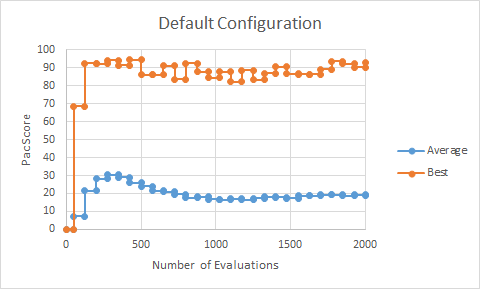
\includegraphics[width=0.8\textwidth]{default}
	\caption{Results of Default Configuration}
\end{figure}

\clearpage

\begin{figure}[h]
	\centering
	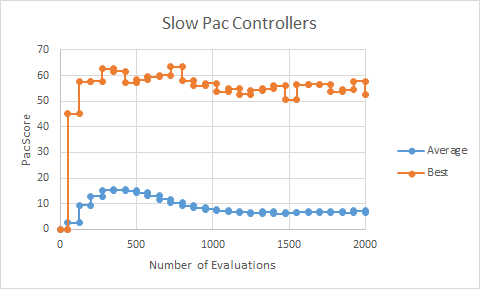
\includegraphics[width=0.8\textwidth]{speedSlow}
	\caption{Results of Slow Pac Controllers}
\end{figure}
\end{flushleft}

\begin{flushleft}
\begin{figure}[h]
	\centering
	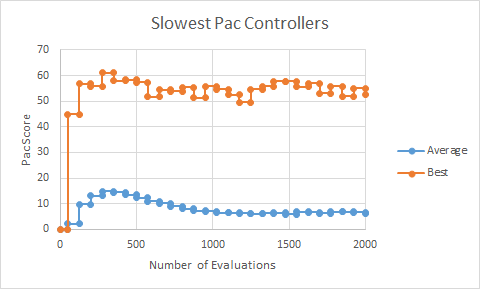
\includegraphics[width=0.8\textwidth]{speedSlowest}
	\caption{Results of Slowest Pac Controllers}
\end{figure}

\clearpage

\begin{figure}[h]
	\centering
	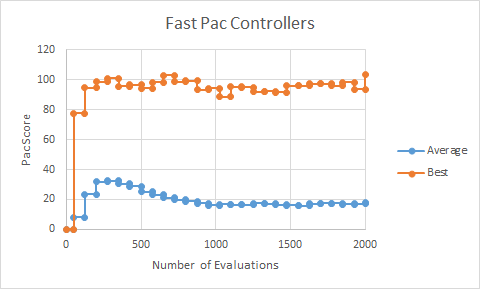
\includegraphics[width=0.8\textwidth]{speedFast}
	\caption{Results of Fast Pac Controllers}
\end{figure}
\end{flushleft}

\begin{flushleft}
\begin{figure}[h]
	\centering
	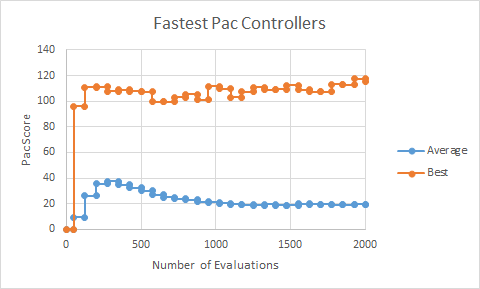
\includegraphics[width=0.8\textwidth]{speedFastest}
	\caption{Results of Fastest Pac Controllers}
\end{figure}

\clearpage

\begin{figure}[h]
	\centering
	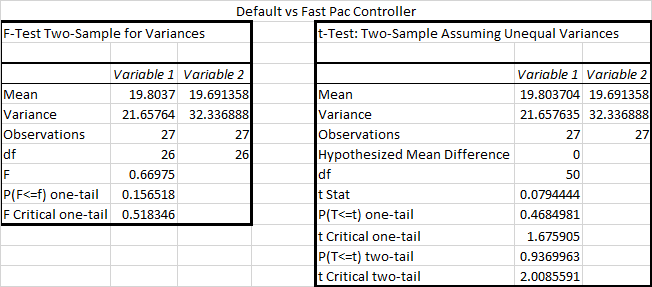
\includegraphics[width=0.8\textwidth]{statDefaultVsFast}
	\caption{Results of Default Configuration vs Fast Pac Controllers}
\end{figure}
\end{flushleft}

\vspace{15mm}

\begin{flushleft}
\begin{figure}[h]
	\centering
	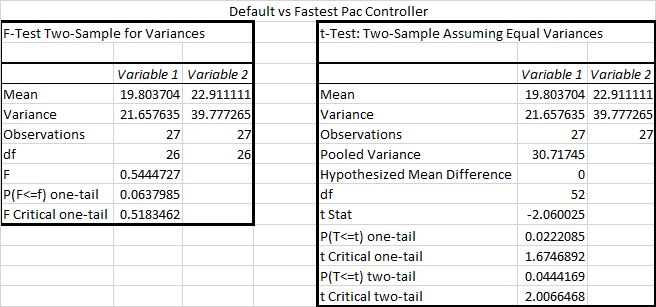
\includegraphics[width=0.8\textwidth]{statDefaultVsFastest}
	\caption{Results of Default Configuration vs Fastest Pac Controllers}
\end{figure}

\clearpage

\begin{figure}[h]
	\centering
	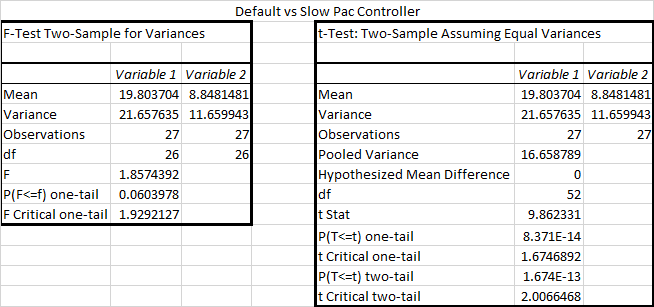
\includegraphics[width=0.8\textwidth]{statDefaultVsSlow}
	\caption{Results of Default Configuration vs Slow Pac Controllers}
\end{figure}
\end{flushleft}

\vspace{15mm}

\begin{flushleft}
\begin{figure}[h]
	\centering
	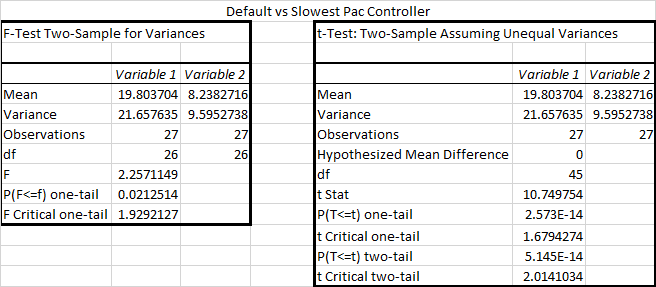
\includegraphics[width=0.8\textwidth]{statDefaultVsSlowest}
	\caption{Results of Default Configuration vs Slowest Pac Controllers}
\end{figure}

\clearpage

\begin{figure}[h]
	\centering
	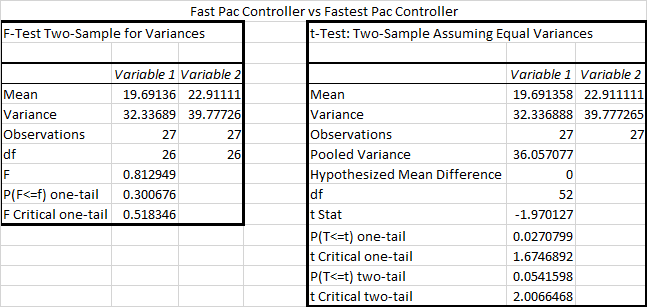
\includegraphics[width=0.8\textwidth]{statsFastVsFastest}
	\caption{Results of Fast Pac Controllers vs Fastest Pac Controllers}
\end{figure}
\end{flushleft}

\vspace{15mm}

\begin{flushleft}
\begin{figure}[h]
	\centering
	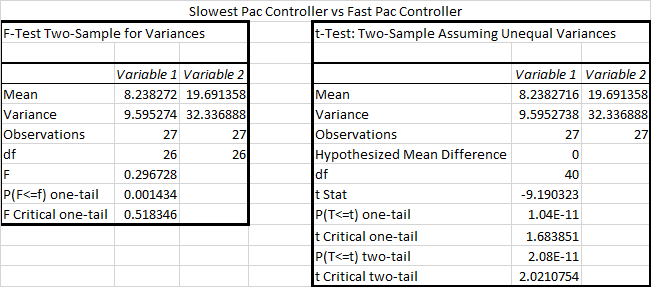
\includegraphics[width=0.8\textwidth]{statsSlowestVsFast}
	\caption{Results of Slowest Pac Controllers vs Fast Pac Controllers}
\end{figure}

\clearpage

\begin{figure}[h]
	\centering
	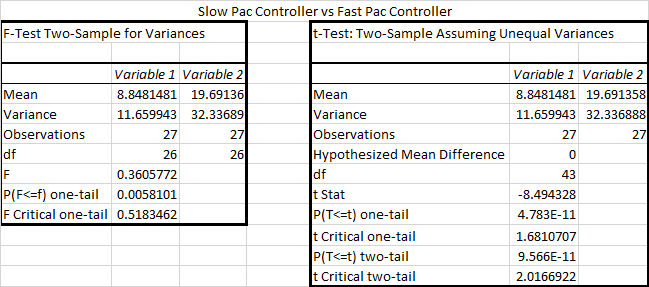
\includegraphics[width=0.8\textwidth]{statsSlowVsFast}
	\caption{Results of Slow Pac Controllers vs Fast Pac Controllers}
\end{figure}
\end{flushleft}

\vspace{15mm}

\begin{flushleft}
\begin{figure}[h]
	\centering
	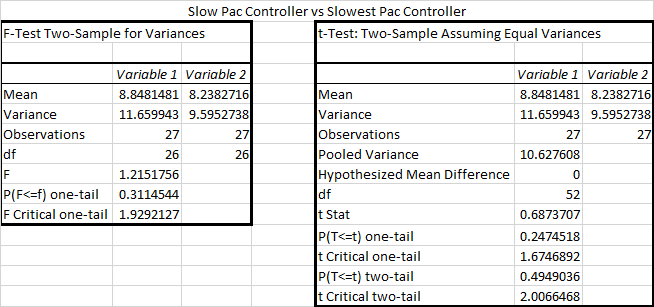
\includegraphics[width=0.8\textwidth]{statsSlowVsSlowest}
	\caption{Results of Slow Pac Controllers vs Slowest Pac Controllers}
\end{figure}
\end{flushleft}

\clearpage
\subsection{Discussion}
\begin{flushleft}
\tab
The mean of the basic configuration is less than the mean of the fast
configuration, and F is greater than F Critical,
so equal variances can be assumed. The absolute value of T stat is less than the
 absolute value of t critical two-tail, so it can not be determined with 95%
 confidence whether either configuration is better.

\tab
The mean of the basic configuration is less than the mean of the fastest
 configuration, and F is greater than F Critical,
 so equal variances can be assumed. The absolute value of T stat is greater
 than the absolute value of t critical two-tail, so it can be stated with 95%
 confidence that using the fastest controllers gives the pac controllers an
 evolutionary advantage compared to the basic configuration.

\tab
The mean of the basic configuration is greater than the mean of the slow
 configuration , and F is less than F Critical,
 so equal variances can be assumed. The absolute value of T stat is greater
 than the absolute value of t critical two-tail, so it can be stated with 95%
 confidence that using slow configurations is an evolutionary disadvantage for
 pac controllers compared to the basic configuration.

\tab
The mean of the basic configuration is greater than the
 mean of the slowest configuration, and F is greater than F
 Critical, so equal variances cannot be assumed. The absolute value of T stat is
 greater than the absolute value of t critical two-tail, so it can be stated
 with 95% confidence that using the slowest configurations is an evolutionary
 disadvantage for pac controllers compared to the basic configuration.

\tab
The mean of the fast configuration is less than the mean
 of the fastest configuration, and F is greater
 than F Critical, so equal variances can be assumed. The absolute value of T stat is less than the
  absolute value of t critical two-tail, so it can not be determined with 95%
  confidence whether either configuration is better.

\tab
The mean of the slowest configuration is less than the mean
 of the fast configuration, and F is less
 than F Critical, so equal variances cannot be assumed. The absolute value of T
 stat is greater than the absolute value of t critical two-tail, so it can be
 stated with 95% confidence that using the slowest pac controllers against unique ghost
 controllers gives a distinct evolutionary advantage to pac controllers that
 the slowest pac controllers do not have.

\tab
The mean of the slowest configuration  is less than the mean
 of the fastest configuration, and F is less
 than F Critical, so equal variances cannot be assumed. The absolute value of T
 stat is greater than the absolute value of t critical two-tail, so it can be
 stated with 95% confidence that the slowest pac controllers are at an
 evolutionary disadvantage compared to the fastest pac controllers.

\tab
The mean of the slow configuration is less than the mean
 of the fast configuration, and F is less
 than F Critical, so equal variances cannot be assumed. The absolute value of T
 stat is greater than the absolute value of t critical two-tail, so it can be
 stated with 95% confidence that using the fast configuration gives pac
 controllers an evolutinary advantage over slow configurations.

\tab
The mean of the slow configuration is less than the mean
 of the fastest configuration, and F is less
 than F Critical, so equal variances cannot be assumed. The absolute value of T
 stat is greater than the absolute value of t critical two-tail, so it can be
 stated with 95% confidence that using the fastest configuration gives pac
 controllers an evolutionary advantage over pac controllers that use the slow
 configuration.

\tab
The mean of the slow configuration is greater than the mean
 of the slowest configuration, and F is less
 than F Critical, so equal variances can be assumed. The absolute value of T
 stat is less than the absolute value of t critical two-tail, so it cannot be
 stated with 95% that either configuration is better than the other.
\end{flushleft}

\subsection{Conclusion}
\begin{flushleft}
Generally, any configuration is not worse than any slower configuration. The
 larger the speed gap, the greater the chance that the faster configuration is
 better. If co-evolution has stagnated, then changing speed is an easy way to
 push up or down a given population.
\end{flushleft}

\end{document}
